\section{Discussion}
% 1 page
From the state of the project at the time of writing, with one week left to deadline, our estimations seem to be more or less correct. Important tasks not anticipated from the start have shown, however, meaning that our task estimations largely holds, but the overall estimation of the required time to finish the project does not.

Beside the extra tasks not initially planned for the backlog, unforeseen problems have occurred on the server we developed doing the first part of the project.
We had foreseen that some errors probably would arise in regards to functionality on the server, but we had no idea what would fail, how much would fail, how long it would take to debug, or how long it would take to fix the errors, if needed.

So far the server errors have been easy to fix, but each time an error has been encountered, time unproportional to the problem itself has been wasted determining whether the error origins from the server or from our newly created client.
This uncertainty is due to poor error reporting facilities, combined with lack of proper testing on the server. The last part only stresses the importance of proper quality assurance.

Though our plans have been subject to delays, the project seems to be back on track. This is suggested by our burndown chart (see figure \ref{burndown} in the appendix) where the lines line up really nicely at the moment. If we are able to continue as currently, we should be able to meet the deadline with all planned functionality implemented for the client.

An important hint at this can also be extracted from the burndown chart, which shows that it is only recently that the project got back on track. This is mainly due to the extra effort which has been needed in order to solve the server problems stated above.
The server and its potential errors should no longer be of much concern since most of the code responsible for communication with the server has been implemented and tested, thereby mainly leaving tasks concerned with creating a functional GUI.

We believe that we have been able to handle the addition of unforseen tasks only because we choose to reserve much more time than we initially estimated to be required. By comparing
the burndown chart with our timetable it is clear that in some periods backlog tasks took about twice the time than estimated to complete them, due to additional, unforseen tasks coming up. Without extra time to perform these unforseen tasks we would currently be far behind schedule.

Beside the code, however, we also have a report to write for the project - a report which at this point hardly has been started, but only have been split into tasks and estimated.
Even though it primarily is the GUI components we have left to do beside the report, extra tasks are bound to origin when considering the project history so far. Still, at this point we have clearly illustrated our ability to catch up with schedule, even when far behind.
It should therefore be possible for us to meet the deadline by just following our plan. In the worst case we will need to downgrade some of the planned functionality or discard the tasks with lowest priority in our backlog.

Having discussed the project, it is also appropriate to discuss the development of how the team as `an organization' developed during the project. To do this, we will evaluate ourselves against the Capability Maturity Model, a model created by the Software Engineering Institute of Carnegie Mellon University, which describes the development process an organization must pass through to be considered mature.

\begin{figure}[t]
  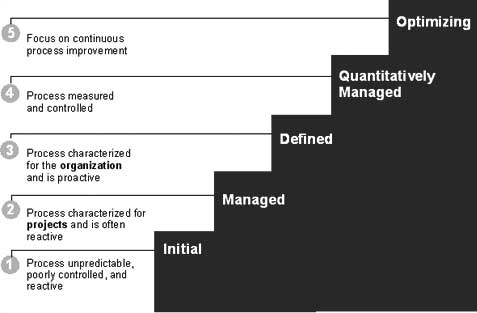
\includegraphics[width=\textwidth]{illustrations/CMM.jpg}
  \caption{The Capability Maturity Model. During the second part of this project we moved from the first level to the second. Source: [\textit{http://www.tutorialspoint.com/cmmi/cmmi-maturity-levels.htm}]}
  \label{fig:Capability_Maturity_Model}
\end{figure}

While doing our project, we moved from the initial level of the Capability Maturity Model (while developing the server) to the managed level (during the development of the client) (see figure \ref{fig:Capability_Maturity_Model}). We kept to the initial level during the first part of the project by developing as we went along without using well-known development methods or initial design. Under the planning and development of the second part of the project we moved to the managed level by using knowledge of our time consumption from them first part of the project, along with some degree of management and progress tracking \cite[p. 242]{PM}. This move up the ladder sheds light on exactly what we want to show in this report, namely that the use of planning methods gives you a huge advantage in producing a product. When not using any of these methods it is highly uncertain that any useful product can be finished on time.
\newpage